

\begin{subsection}{Internode communication}

\begin{frame}
 \begin{block}{How does information (dynamic content) move around?}
 Using the same routing and incentive system as storage and retrieval.
 \end{block}
\end{frame}


\begin{frame}{Internode communication}
\begin{block}{What kinds of interactions are we used to?}
 \begin{itemize}
    \item tweets, status updates (public or restricted)
    \item chatroom, discussion forum, stackoverflow
    \item pager \& fax, phonecall, videocall
    \item audio-video broadcast, tv, radio, podcast (live or recorded)
    \item rss, subscription, notifications, newsletters
    \item file transfer, download
 \end{itemize}
\end{block}
\begin{block}<2->{Question:}
 Why are these services provided by private entities and are not part of the basic public infrastructure? After all, everything is just pulling, pushing and storing data.
\end{block}
\end{frame}

\begin{frame}
\setbeamercovered{transparent}% Dim out "inactive" elements
\begin{overlayarea}{\textwidth}{10cm}
To replicate services we are used to, specify storage and delivery criteria.
\begin{block}{}
 \begin{itemize}
  \item<2-> Who is it for?
  \item<3-> How should it be stored and transported?
  \item<4-> Encryption?
  \item<5-> What is the context?
 \end{itemize}
\end{block}
 \only<2->{
\begin{block}<2->{}
\begin{itemize}
  \only<2>{
    \item Is it addressed to specific recipients?
    \item Should it be (re-)delivered to specific recipients?
    }
 \only<3>{
    \item Should it be stored (at content address) or is it ephemeral?
    \item Does it have high priority, is it urgent, is latency a factor?
    \item Should it be archived? is it insured? expiring?
    \item Is data access recorded/receipted?
    }
 \only<4>{
    \item Is it confidential? Private?
    }
 \only<5>{
    \item reaction to previous communication, content, topic? Comments, answers, corrections
    \item Existing asset (reference), streaming data, real time feed?
    \item How should the data be displayed? Timeline or thematic/threaded view
    }
\end{itemize}
\end{block}
}
\end{overlayarea}
\end{frame}


\begin{frame}
 \begin{block}{The Vision}
Use the message routing and content delivery system that swarm uses
 \end{block}
 \begin{block}<2->{Tools at our disposal}
  \begin{itemize}
   \item incentivised message relay (store requests sent towards non-content address must be paid for)
   \item deterministic routing and message delivery (to complement Whisper)
   \item priority queues
   \item insured storage
   \item taking receipts
   \item multicast broadcast
  \end{itemize}
 \end{block}
\end{frame}

\wholeslide{\textbf{PSS}: \textbf{P}ostal \textbf{S}ervices \textbf{S}uite (BZZ-whispered)}

\end{subsection}

\begin{subsection}{Multimedia live broadcast}

\blockslide{}{How can this handle live multimedia sessions?}

\begin{frame}{}
\begin{block}{Multimedia live broadcast: multibitrate low-latency streaming}
 \begin{itemize}
    \item leech - continuous data stream from peers
    \item non-multiplexed multi-bitrate stream offered
    \item RTSP/MPEG-DASH standard - available in most browsers using html5 video tag
    \item webRTC or FFMEG to capture and encode streams
    \item multicast tree - solves scalability of media server solutions
    \item p2p symmetry: the same technique for videoconference or even one-on-one AV session
    \item data goes to viewers via pairwise transmission channels
    \item peers sit on the multicast chain and get  promoted, demoted depending on payment and latency/throughput
    \item the same framework can drive historical syncing
\end{itemize}
\end{block}
\end{frame}

\wholeslide{\textbf{SWATCH}: \textbf{S}treaming \textbf{W}ith \textbf{A}daptive \textbf{T}ransmission \textbf{CH}annels}

\end{subsection}

\begin{subsection}{Database services}


\begin{frame}
\begin{block}{Where is information (dynamic content) pulled from?}
\begin{enumerate}
\item the blockchain, ethereum state \& contract storage. (expensive and slow)
\item local storage private to user, cookies (limited to data only client uses)
\item distributed database on swarm? (cheap and verifiable)
\end{enumerate}
\end{block}
\end{frame}

\begin{frame}
\setbeamercovered{transparent}% Dim out "inactive" elements
\begin{overlayarea}{\textwidth}{10cm}
\begin{block}{How are database services organised?}
\begin{itemize}
\item<1-> Structure
\item<2-> Security
\item<3-> Scalability
\item<4-> Sustainability
\end{itemize}
\end{block}
\begin{block}{How?}
\begin{itemize}
\only<1>{
\item manifests implement key-value store (Patricia Merkle Trie as oppose to traditional DHT)
\item supports various indexes and iteration (range queries)
\item conventions for index entry
\item db table layout manifest
\item linked to ENS
}
\only<2>{
\item  verifiable on the blockchain by challange so it does not have to be on-chain
\item  verifiable authentication, record updates and notifications
}
\only<3>
{
\item sql resolver (reql of rethinkdb) sitting on top
\item parallel processess walk the indexes and merge results
\item index updates, derivative data (full text search indexes, aggregate statistics) supplied by a computational market
\item query caching and accelerated retrieval for real-time low latency experience supplied by specialised nodes
}
\only<4>
{q
\item due to verifiable computations (truebit, ewasm), \textit{swap, swear and swindle} is applicable
\end{itemize}
\end{block}
\begin{block}{Examples}
\begin{itemize}
\item example: decentralised markets
\item example: storing the blockchain and state on swarm
}
\end{itemize}
\end{block}
\end{overlayarea}
\end{frame}

\wholeslide{\textbf{SWORD}: \textbf{S}tate \textbf{W}ith \textbf{O}n-demand \textbf{R}etrieval of \textbf{D}ata}


\begin{frame}
\begin{block}{Can we put the ethereum blockchain and state on swarm}
\begin{itemize}
 \item light client, LES protocol abstraction - flexible transition from remote, light, full and archival nodes
 \item solves the scalability problem of too big state data, receipts, contract storage, fast syncing
 \item decentralised blockchain explorer
\end{itemize}
\end{block}
\end{frame}

\end{subsection}



\begin{subsection}{Current Status}
\begin{frame}[plain]
 \begin{tikzpicture}
  \node[scale=1]{
  \begin{tikzpicture}
  \node[anchor=center] at (current page.center) (thepic){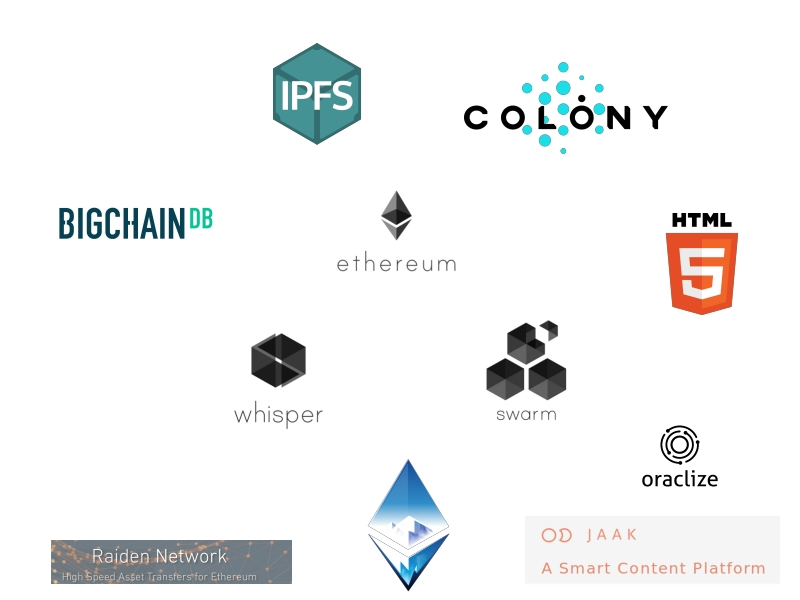
\includegraphics[width=0.9\textwidth]{ecosystem1.jpg}};
  \node[below=1cm of thepic.130] {\textbf{PSS}};
  \node[below=5cm of thepic.135] {\textbf{ENS}};
  \node[below=2.7cm of thepic.65] {\textbf{SWATCH}};
  \end{tikzpicture}
 };
 \end{tikzpicture}

\end{frame}


\begin{frame}{Ethereum: status and roadmap}
 \begin{block}{Current Status}
 `Homestead' up and running. Multiple client implementations.
 \end{block}
 \begin{block}{Roadmap}
  `Metropolis' release milestone\\
  `Mist browser' - Dapp browser with swarm support.
 \end{block}

\end{frame}


\begin{frame}{Swarm: status and usage}
\begin{block}<1->{What is the developlent status of swarm?}
\begin{enumerate}
\item golang implementation: proof-of-concept iteration 2 release 4, code has been merged to go-ethereum develop branch
\item Microsoft Azure hosting a testnet of 100+ nodes
\item expanding team, come join or contribute
\end{enumerate}
\end{block}

\begin{block}<2->{How can swarm be used?}
\begin{itemize}
\item bzzd - swarm daemon, communicates with ethereum via IPC, so any ethereum client works
\item APIs: JSON RPC (via websockets, http, or ipc), http proxy, cli, fuse driver (planned)
\item API bindings: web3.js and CLI
\end{itemize}
\end{block}

\end{frame}

\begin{frame}
\begin{overlayarea}{\textwidth}{10cm}
\begin{tikzpicture}
\node[scale=0.8] at (current page.center) {
\begin{tikzpicture}

 \node[draw,rounded corners] at (4,4) (goapi) {
\includegraphics[width=2cm]{golang.png} API};

 \node[draw,rounded corners] at (0,0) (ipc) {JSON IPC};
 \node[draw,rounded corners] at (4,0) (proxy) {http-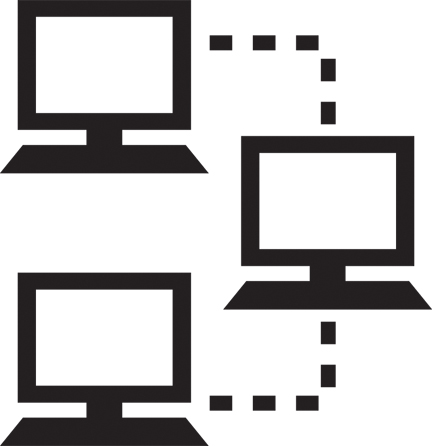
\includegraphics[width=1cm]{proxy.jpg}-proxy};
 \node[draw,rounded corners] at (8,0) (fuse) {fuse 
\includegraphics[width=1cm]{fuse.jpg}};

 \node[draw,rounded corners] at (2,-4) (cli) {CLI 
\includegraphics[width=1cm]{cli.png}};
 \node[draw,rounded corners] at (6,-4) (web3js) {web3.js};

 \node {}
 (cli) edge[point,->] (ipc)
 (web3js) edge[point,->] (ipc)
 (cli) edge[point,->] (proxy)
 (web3js) edge[point,->] (proxy)
 (cli) edge[point,->] (fuse)
 (web3js) edge[point,->] (fuse)
 (ipc) edge[point,->] (goapi)
 (proxy) edge[point,->] (goapi)
 (fuse) edge[point,->] (goapi)
 ;
\end{tikzpicture}
};
\end{tikzpicture}
\end{overlayarea}
\end{frame}

\end{subsection}


